% -----------------------------------------------------------------------------
\section{Source typologies}
An OpenQuake PSHA input model contains a number of sources belonging 
to a finite set of possible typologies. Currently OpenQuake supports 
four seismic source types. Each type contains a limited number of 
parameters necessary to specify geometry and seismicity occurrence. 

In the following sections we provide a detailed description of the 
source typologies currently supported by OpenQuake and that can be 
included in an Initial Seismic Sources Model as explained in the 
introduction of this chapter and in Section \ref{hazard:pshainputmodel}.
%
%  - - - - - - - - - - - - - - - - - - - - - - - - - - - - - - - - - - - - - - -
\subsection{Seismic source typologies description}
\label{sec:seismic_source_descr}
%
OpenQuake, at present time, provides four seismic source typologies, 
for the most part defined in the GEM1 project \citep{pagani2010}. 
%
The main seismic source types currently supported are the following:
\begin{itemize}
\item Area source - So far, the most frequently adopted source 
type in national and regional PSHA models.
\item Grid sources - Grid sources can be considered a replacement 
for area sources since they both model distributed seismicity;
\item Simple fault - A Simple fault is the easiest way to
specify a fault source in OpenQuake. This typology is habitually adopted 
to describe shallow seismogenic fault sources.
\item Complex fault - A complex fault is more often used 
to model subduction interface sources with a complex geometry. 
\end{itemize}

These are the basic assumptions accepted in the definition of these source 
typologies:
\begin{itemize}
\item In the case of area and fault sources, the seismicity is homogeneously 
distributed over the source; 
\item Seismicity temporal occurrence follows a Poissonian model; 
\item The frequency-magnitude distribution distribution can be approximated 
to an evenly discretized distribution. 
\end{itemize}
%
%  . . . . . . . . . . . . . . . . . . . . . . . . . . . . . . . . . . . . . . . 
\subsubsection{Area sources}
\label{hazard:seismic_source_types:areaSources}
\index{Source type!area} 
\index{Area source|see{Source type}}
%
Area sources model the seismicity occurring over wide areas where  
identification or characterization - i.e. unambiguous definition 
of seismicity occurrence parameters - of single sources is difficult. 
%
The \citet{sshac1997} - using as a discriminant the extension - 
defined three main types of area seismic sources:
\begin{enumerate}
\item Area sources enclosing concentrated zones of seismicity;
\item Regional area sources;
\item Background area sources.
\end{enumerate}
%
The criteria adopted for their definition - and the related 
uncertainties - vary according to each area source type. 
%
From a computation standpoint we do not introduce any difference 
between these three area types.
%
%  . . . . . . . . . . . . . . . . . . . . . . . . . . . . . . . . . . . . . . . 
\paragraph{Parameters}
\begin{itemize}
\item A polygon that identifies the external border of the area. 
The current version of OQ doesn't support the definition 
of internal borders
\item One (or several) combinations of the following objects:
\begin{itemize}
	\item A discrete frequency-magnitude distribution 
	\item (optional) Strike, dip, and rake angles indicating 
	main fault geometry and slip direction for the seismicity  
	in the corresponding FMD.
	%
	For example, in the PSHA model prepared within the PEGASUS project,
	\cite{coppersmith2009} defines for each area source a discrete 
	distribution of strike values (dip is not considered because the 
	source-site metrics they use is the Joyner-Boore distance). 
\end{itemize}
%
This description permits the accurate characterization of seismicity 
occurrence within an area by explicitly taking into account the existing 
faulting trends. 
%
\item An array specifying the depth to the top of rupture dependency on 
magnitude. The array contains two columns and as many rows as the 
number of $<$depth, magnitude$>$ tuples used. 
The depth in each tuple defines the top of rupture for magnitudes equal 
or greater than the corresponding value. 
%
\item A value to indicate the hypocentral depth in case of punctual sources. 
By convention all the events with magnitude lower than the lowest value of 
magnitude contained in the depth to the top of rupture array are modelled as 
punctual sources. 
%
On the opposite, ruptures with magnitude equal or greater than 
the lowest value of magnitude contained in the depth to the top of rupture array 
are modelled considering their finite dimensions. The finite dimension of the 
rupture is computed using a magnitude-area or magnitude-length relationship 
specified in the calculation settings file (in future versions of OQ we will 
allow the user to specify for each tectonic region the corresponding 
magnitude-scaling relationship).
\end{itemize}
%
%  . . . . . . . . . . . . . . . . . . . . . . . . . . . . . . . . . . . . . . .
\subsubsection{Grid sources}
\label{hazard:seismic_source_types:gridSources}
\index{Source type!grid}
\index{Grid source|see{Source type}}
A grid source  is a typology used to model distributed seismicity - usually 
of low and intermediate magnitude.
%
Grid sources can be considered a PSHA source model alternative to area 
sources, since they both try to represent distributed seismicity. Grid sources 
usually derive from the application of seismicity smoothing algorithms 
\citep{frankel1995,woo1996}. 
%
The use of these algorithms carries some advantages compared to area sources, 
indeed, (1) they remove most of the unavoidable degree of subjectivity due to 
the definition of the geometries and (2) they define a seismicity spatial 
pattern that is, usually, more similar to reality. Nevertheless, some smoothing 
algorithms require the a-priori definition of some setup parameters that expose 
the calculation to a certain partiality level.

Grid sources are modelled in OpenQuake simply as a set of 
point sources. The next section describes the parameters required to 
characterize a point source.
%
%  . . . . . . . . . . . . . . . . . . . . . . . . . . . . . . . . . . . . . . . 
\paragraph{Parameters}
%
For each grid node:
\begin{itemize}
\item A location specified in terms of the $<$latitude,longitude$>$ tuple;
\item Similarly to area sources, one (or many) combinations of the following 
objects:
	\begin{itemize}
	\item A discrete frequency-magnitude distribution
	\item Strike, dip, and rake angles characterizing the seismicity 
	specified in the associated FMD. 
	\end{itemize}
\item An array to specify the dependency on magnitude of the depth to 
	the top of rupture. This array contains two columns and one or many 
	$<$depth, magnitude$>$ tuples where each tuple specifies the depth to the 
	top of rupture for magnitudes equal or greater than a specific value. 
\item A value to indicate the hypocentral depth in case of punctual sources. 
	The same convention specified for area sources applies here. 
\end{itemize} 
%
%  . . . . . . . . . . . . . . . . . . . . . . . . . . . . . . . . . . . . . . .
\subsubsection{Simple faults}
\index{Source type!fault!simple geometry} 
\index{Simple fault|see{Source type}}
%
Simple Faults are the most common source type used to model faults; the 
``simple'' adjective relates to the geometry description of the source 
which is basically obtained by projecting a trace (i.e. a polyline) along 
a representative dip direction. 
%
%  .   .   .   .   .   .   .   .   .   .   .   .   .   .   .   .   .   .   .   . 
\paragraph{Parameters}
%
\begin{itemize}
\item A fault trace (usually a polyline); 
\item A discrete frequency-magnitude distribution
\item A representative value of the dip angle (specified according to 
the Aki-Richards convention; see \citet{aki2002});
\item Rake angle (specified following the Aki-Richards convention; 
see \citet{aki2002}) 
\item Upper and lower values of depth limiting the seismogenic interval 
\item A boolean flag that specifies if the size of ruptures should 
follow a magnitude scaling relationship (currently specified in the 
calculation settings file) and be distributed homogeneously over the 
fault surface or it is accepted that ruptures within a given range of 
magnitudes (specified by the FMD) will always rupture the entire fault 
surface.
\end{itemize}
%
%  . . . . . . . . . . . . . . . . . . . . . . . . . . . . . . . . . . . . . . .
\subsubsection{Complex faults}
\index{Source type!fault!complex geometry}
\index{Complex fault|see{Source type}}
%
Complex faults  differ from simple fault just by the way geometry is 
described and, consequently in the way the fault surface is created. The 
input parameters used to describe complex faults are, for the most part, 
the same used to describe the simple fault typology. In particular, in 
the case of complex faults the dip angle is not requested while the fault
trace is substituted by two fault traces used to limit at top and bottom 
the fault surface. 
%
Usually, we use complex faults to model intraplate megathrust faults such 
as the big subduction structures active in the Pacific (Sumatra, South 
America, Japan).

% -----------------------------------------------------------------------------
\section{Calculation workflows}
% Three types of analysis
The hazard component of OpenQuake-Hazard performs seismic hazard 
analysis (SHA) following various approaches. 
%
Currently three main types of analysis are supported:
\begin{itemize}
\item \textit{Classical Probabilistic Seismic Hazard Analysis (cPSHA)}, 
allowing calculation of hazard curves and hazard maps following the 
classical integration procedure 
(\cite{cornell1968}, \citet{mcguire1976}) as formulated by \cite{field2003}).
\item \textit{Event-Based Probabilistic Seismic Hazard Analysis (ePSHA)}, 
allowing calculation of ground-motion fields from stochastic event sets. 
Eventually, classical cPSHA results - such as hazard curves - can be 
obtained by post-processing the set of computed ground-motion fields.
\item \textit{Deterministic SHA (DSHA)}, allowing calculation of ground 
motion fields from a single earthquake rupture scenario taking into account 
ground-motion aleatory variability.
\end{itemize}
Each of these analysis types has a modular structure, which provides the capability of investigating 
all possible intermediate results. Moreover, each calculator can be 
extended independently of the others so that more calculation 
options and methodologies can be easily introduced, without affecting the 
overall calculation workflow. 
Each of the workflows described in the following Sections involves a number 
of calculators, each responsible for a specific task. 
Figures \ref{classical_psha_workflow}, \ref{event_based_workflow}, and 
\ref{deterministic_workflow} schematically depict the different calculation 
workflows.
%
%  - - - - - - - - - - - - - - - - - - - - - - - - - - - - - - - - - - - - - - -
\subsection{Classical Probabilistic Seismic Hazard Analysis}
\label{section:classicalPSHA}
%
Input data for the classical PSHA consist of a PSHA Input Model (PSHAim) that 
is provided together with a set of calculation settings. 
%
The OpenQuake book \citep{crowley2011} describes extensively the content of a PSHAim and 
- in particular - the different options for modeling seismogenic sources 
and the option offered to include epistemic uncertainties on both seismicity 
and ground-motion models in the form of a logic tree.
%
% ..............................................................................
% . . . . . . . . . . . . . . . . . . . . . . . . . . . . . . . . . . . > Figure
\begin{figure}[htbp]
\begin{center}
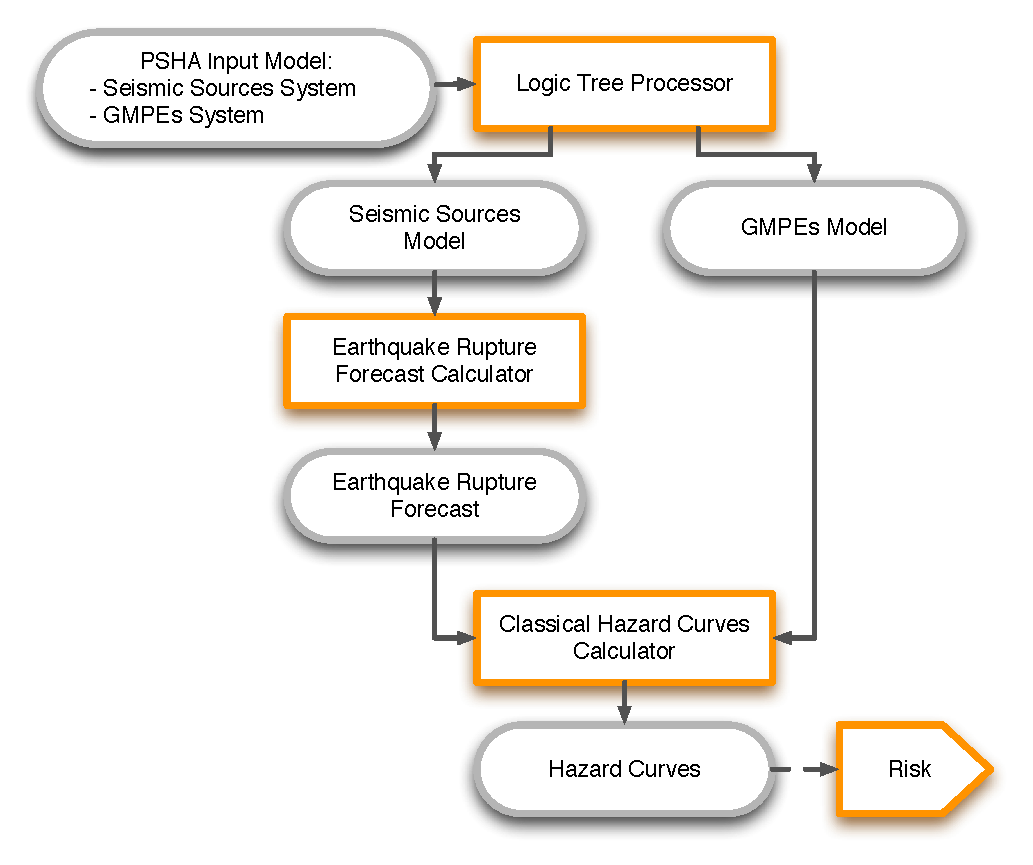
\includegraphics[width=14cm]{./figures/classical_psha_workflow.eps}
\caption{Workflow for classical PSHA (boxes with an orange border represent the 
calculators). Given a PSHA Input Model 
the Logic Tree Processor is responsible for creating a Seismic Source model
and a ground-motion model. 
The Seismic Source model is then provided to the Earthquake Rupture Forecast 
calculator, which computes the ERF (the list of all earthquake ruptures in the 
source model with their probabilities of occurrence). 
Using the ERF and the GMPEs model the Classical PSHA calculator produces 
curves at the sites of interest.}
\label{classical_psha_workflow}
\end{center}
\end{figure}
% . . . . . . . . . . . . . . . . . . . . . . . . . . . . . . . . . . . < Figure
% ..............................................................................

As represented in Figure \ref{classical_psha_workflow}, the main calculators 
used to perform this analysis are:
\begin{enumerate}
%
\item \emph{Logic Tree Processor} \hfill \\
The Logic Tree Processor (LTP) takes as an input the PSHA Input Model and 
creates a Seismic Source Model. The LTP uses the information in the Initial 
Seismic Source Models and by 'harvesting' the information contained in the 
Seismic Source Logic Tree - that is to sample the epistemic uncertainties - 
it creates a Seismic Source Model (i.e. a model describing geometry and 
activity rates of each source without any epistemic uncertainty). 
%
Following the procedure just described the Logic Tree Processor creates a 
Ground Motion model (i.e. a data structure that associates to each tectonic 
region considered in the calculation a GMPE).
%
\item \emph{Earthquake Rupture Forecast Calculator} \hfill \\
The produced Seismic Source Model is then used as input for the Earthquake 
Rupture Forecast (ERF) calculator which computes the probability of occurrence, 
over a specified time span, for each earthquake rupture produced by the source 
model.
\item \emph{Classical PSHA Calculator} \hfill \\
The cPSHA uses the ERF and the Ground Motion model to compute hazard curves on 
each site specified in the calculation settings.
\end{enumerate} 
%
%  - - - - - - - - - - - - - - - - - - - - - - - - - - - - - - - - - - - - - - -
\subsection{Event-Based Probabilistic Seismic Hazard Analysis}
\label{section:event-basedPSHA}
Input data for the Event-Based PSHA - as in the case of the Classical PSHA 
calculator - consist of a PSHA Input Model supplied to OQ together with a 
set of calculation settings.
%
% ..............................................................................
% . . . . . . . . . . . . . . . . . . . . . . . . . . . . . . . . . . . > Figure
\begin{figure}
\centering
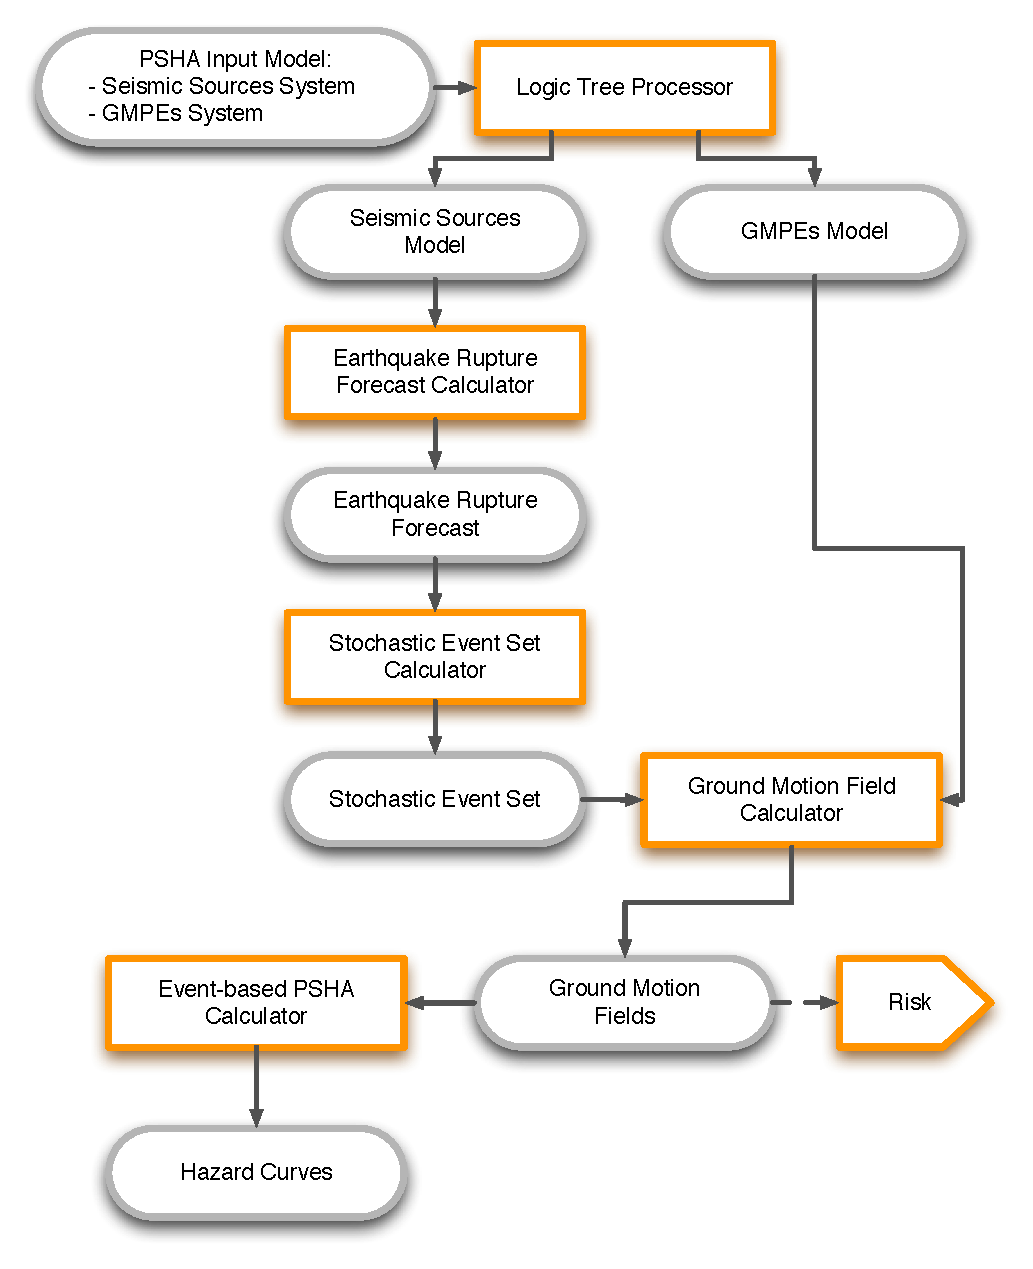
\includegraphics[width=14cm]{./figures/event_based_workflow.eps}
\caption{Workflow for event-based PSHA. Similar to the classical PSHA workflow 
(Figure \ref{classical_psha_workflow}), an ERF is computed, which is then used 
to generate a stochastic event set (representative of the seismic activity of 
a region in a given time span). Each event is then utilized to calculate a 
ground-motion field over a region of interest.}
\label{event_based_workflow}
\end{figure}
% . . . . . . . . . . . . . . . . . . . . . . . . . . . . . . . . . . . < Figure
% ..............................................................................
As represented in Figure \ref{event_based_workflow}, the main calculators 
used to perform this analysis are:
\begin{enumerate}
%
\item \emph{Logic Tree Processor} \hfill \\
The Logic Tree Processor was already 
introduced in the description of the cPSHA workflow (see section 
\ref{section:classicalPSHA} at page \pageref{section:classicalPSHA}).
%
\item \emph{Earthquake Rupture Forecast Calculator} \hfill \\ 
The Earthquake Rupture Forecast Calculator was already 
introduced in the description of the cPSHA workflow (see section 
\ref{section:classicalPSHA} at page \pageref{section:classicalPSHA}).
%
\item \emph{Stochastic Event Set Calculator} \hfill \\
The Stochastic Event Set Calculator generates a Stochastic Event set 
by sampling each rupture contained in the ERF according to its 
probability of occurrence. Usually a Stochastic Event Set (SES) contains
a large number of seismicity histories each one representative of a  
possible collection of events that can be produced by the seismic source
considered in an analysis during the time span fixed for the calculation
of hazard (normally corresponding to 50 years).
%
\item \emph{Ground Motion Field Calculator} \hfill \\
The Ground Motion Field Calculator computes for each event contained in a 
Stochastic Event Set - provided as an input - a realization of the 
ground shaking taking into account the aleatory uncertainties in 
the ground-motion model. Eventually, the Ground Motion Field calculator 
can consider the spatial correlation of the ground-motion during the 
generation of the GMF.
%
\item \emph{Event-based PSHA Calculator} \hfill \\
The event-based PSHA calculator takes a (large) set of ground-motion 
fields representative of the possible shaking that the investigated 
area can eventually experience over a (large) time span and for each 
grid node in a ground-motion fields computes the corresponding hazard 
curve. 
%
This procedure is computationally intensive and is not recommended for 
investigating the hazard over large areas. 
\end{enumerate}

The Logic Tree Processor and the Earthquake rupture forecast were already 
introduced during the descrption of the cPSHA workflow (see section 
\ref{section:classicalPSHA} at page \pageref{section:classicalPSHA}).
%
%  - - - - - - - - - - - - - - - - - - - - - - - - - - - - - - - - - - - - - - -
\subsection{Deterministic Seismic Hazard Analysis}
\label{section:deterministicSHA}
% Deterministic
For deterministic SHA (DSHA), the input data consist of a single earthquake 
rupture model and a single ground-motion model. Using the Ground Motion Field 
Calculator, multiple realizations of ground shaking can be computed, each 
realization sampling the aleatory uncertainties in the ground-motion model.

As represented in Figure \ref{deterministic_workflow}, the main calculators 
used to perform this analysis are:
\begin{enumerate}
\item \emph{Ground Motion Field Calculator} \hfill \\
The Ground Motion Field Calculator was already 
introduced during the descrption of the ePSHA workflow (see section 
\ref{section:event-basedPSHA} at page \pageref{section:classicalPSHA}).
\end{enumerate}
% ..............................................................................
% . . . . . . . . . . . . . . . . . . . . . . . . . . . . . . . . . . . > Figure
\begin{figure}[!hb]
\centering
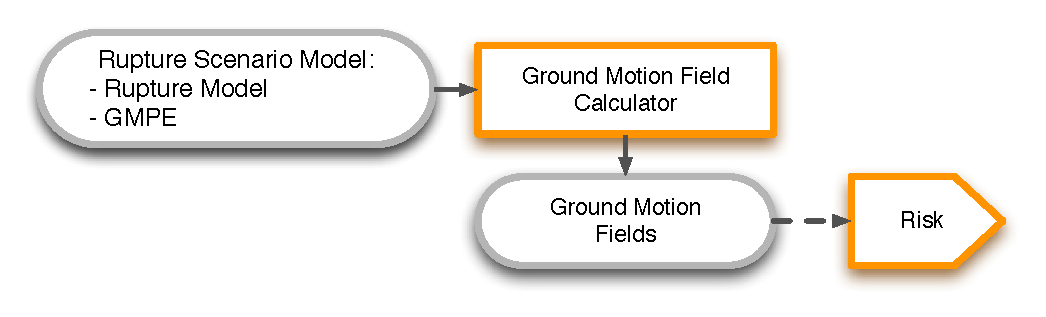
\includegraphics[width=14cm]{./figures/deterministic_workflow.eps}
\caption{Workflow for deterministic SHA. Given a rupture scenario model, 
consisting of an earthquake rupture model, plus a GMPE, the ground-motion 
field calculator can compute multiple ground-motion field realizations (by 
taking into account GMPE aleatory uncertainties).}
\label{deterministic_workflow}
\end{figure}
% ..............................................................................



\cleardoublepage
